% file siminos/froehlich/flotsamFrCv11
% $Author: predrag $ $Date: 2011-01-24 00:23:46 -0500 (Mon, 24 Jan 2011) $

% formerly called by siminos/froehlich/slice/FrCv11.tex

\section{Flotsam from slice article FrCv11}
\label{sec:flotsam}

%\ifboyscout
%\subsubsection{Subsubsection header}
%[Just checking what the header looks like]
%\else
%\fi

---
  %
  %
\PC{{\bf to Stefan}:
write abstract, intro, conclusions often!
This might be the only part of this text that most
people glance at.
%PC 2010-09-30: planted an error into the abstract, just to see how
%   often do you edit it.
%
%
   When you write a project report or a research article, you always
   write abstract, introduction and conclusions first, and then keep
   rewriting them often. They are the most important parts of the text,
   as that is for most people only parts they will look at.
   }

													\toCB

-------------

{\bf PC}{ still have to derive the general case: ``
Let $\sliceTan{}$ be a vector normal to the plane of the slice. Then the
dynamics within the slice are given by
\bea
\dot{\gSpace_a}(\sspRed) &=& \frac{\braket{\vel(\sspRed)}{\sliceTan{a}}}
               {\braket{\groupTan(\sspRed)}{\sliceTan{}}}
\continue
\velRed(\sspRed) &=& \vel(\sspRed)
   -\dot{\gSpace}(\sspRed) \cdot \groupTan(\sspRed)
\label{SF:sliceEas}
\eea
where $\velRed(\sspRed)$ is the velocity in the slice.
    ''}

  %
We only care about those that are local (and preferably global) {\em
minima}, for which all the eigenvalues of the symmetric matrix
$[N\!\times\!N]$ matrix of second derivatives of distance,
\beq
\frac{\partial^2}
     {\partial \gSpace_a \partial \gSpace_b}
        |\sspRed - \slicep|^2
    =
%  - \braket{\Lg_a e^{\gSpace \cdot \Lg} \ssp}{\sliceTan{b}}=
  - \braket{\groupTan_a(\sspRed)}{\sliceTan{b}}=
  \braket{\sspRed}{\Lg_a \Lg_b\slicep}
\ee{PCinflPoint}
are positive. In practice we do not need to actually compute
this matrix, we simply pick from among the local minima
the infimum of the distance.

{\bf PC:}{ could it be that inflections are generic only for \SOn{2},
        but of higher codimension and thus not encountered
        by 1\dmn\ time trajectory for higher-dimensional Lie groups?}

-------------

Most of the Lie groups that we will only be considering here are
compact.

The $L^2$ norm of $\groupTan(u)$ is weighted by
the quadratic Casimir \refeq{QuadCasimir}. For \SOn{2} this is
$C_2^{(m)} = m^2$,
\beq
\oint \frac{d\gSpace}{2\pi}
     \, (\Lg u(\gSpace))^T \Lg u(2\pi-\gSpace)
= \sum_{m=1}^\infty m^2 \left(a_m^2 + b_m^2\right)
\,.
\ee{tangL2norm}


-------------




%\ES{ If find this derivation confusing and hard to follow,
%although it illustrates a very simple fact, encapsulated in this last sentence.
%Contrary to what you say here, in your derivation you start by rotating
%the template $\slicep$, but then also rotate the \statesp\ point $\ssp$ and you
%tacitly use the fact that in order to minimize distance either way you have
%to rotate by the same angle. I don't disagree, but it might be hard for the
%casual reader to follow. I propose the following simplification of the
%derivation, in the spirit of your last sentence: Look instead for minima of
%\[
%	|\LieEl(\gSpace)x-\slicep|^2\,,	
%\]
%to get
%\[
% \frac{\partial ~~}{\partial \gSpace_a}	|\LieEl(\gSpace)x-\slicep|^2 \sim
%		\braket{\Lg_{a}\sspRed}{\sspRed-\slicep}=0\,,
%\]
%and finally use antisymmetry of $\Lg_{a}$ (twice) to write this as
%$\braket{\sspRed}{\sliceTan{a}} =0$.
%
%I also suggest that it might benefit the reader to introduce the group
%angle parameterization earlier in this section, \ie\ use
%$\LieEl(\gSpace)\ssp$ instead of $\LieEl\ssp$, \etc
%}

-------------


Symmetry strongly constrains the form of solutions and their
bifurcations, if appropriately implemented, it can significantly
accelerate convergence of numerical algorithms, it splits the dynamical
\statesp\ into chains of lower-dimensional flow-invariant subspaces,
dictates its invariant partitions and the symbolic dynamics.

-------------

Ridges are of Lebesgue measure zero, no way you would hit them.

We do not need to be very precise about the instant
where we switch, as long as we are away from either slice's singularity
subspace.

-------------

{\bf PC to Stefan}:
	While `fixes' is a correctly used math word, I tend to avoid it 	
as it violates the common usage; $\Lg_1$ does not (transitively) `fix'
anything, 	it simply does not act upon $b$ coordinates.

-------------

 %% ReducTraj*.* - read dasbuch/book/FigSrc/inkscape/00ReadMe.txt
 \begin{figure}
 \begin{center}
  \setlength{\unitlength}{0.40\textwidth}
  %% \unitlength = units used in the Picture Environment
  \begin{picture}(1,0.8361641)%
    \put(0,0){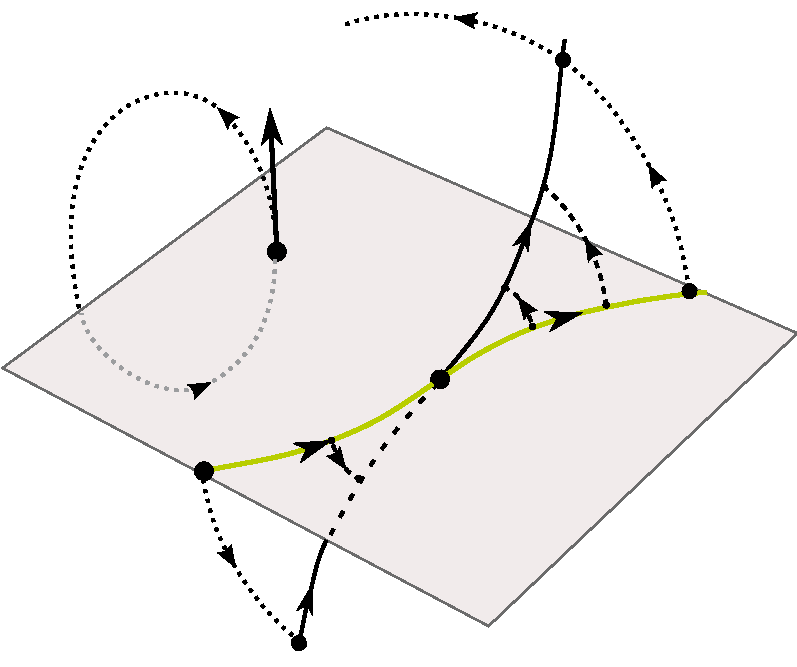
\includegraphics[width=\unitlength]{ReducTraj5.pdf}}%
    \put(0.09054399,0.38282057){\color[rgb]{0,0,0}\rotatebox{-30.34758661}{\makebox(0,0)[lb]{\smash{$\pSRed$}}}}%
    \put(0.57768586,0.29773425){\color[rgb]{0,0,0}\rotatebox{0.0313674}{\makebox(0,0)[lb]{\smash{$\sspRed(0)$}}}}%
    \put(0.59310014,0.69932675){\color[rgb]{0,0,0}\rotatebox{0.03136739}{\makebox(0,0)[lb]{\smash{$\ssp(\tau)$}}}}%
    \put(0.8268425,0.39772328){\color[rgb]{0,0,0}\rotatebox{0.03136739}{\makebox(0,0)[lb]{\smash{$\sspRed(\tau)$}}}}%
    \put(0.81220962,0.66529577){\color[rgb]{0,0,0}\rotatebox{0.03136739}{\makebox(0,0)[lb]{\smash{$\LieEl(\tau)$}}}}%
    \put(0.23150193,0.63610779){\color[rgb]{0,0,0}\rotatebox{0.0313674}{\makebox(0,0)[lb]{\smash{$\LieEl\,\slicep$}}}}%
    \put(0.37740434,0.49597258){\color[rgb]{0,0,0}\rotatebox{0.0313674}{\makebox(0,0)[lb]{\smash{$\slicep$}}}}%
    \put(0.3627714,0.69665188){\color[rgb]{0,0,0}\rotatebox{0.0313674}{\makebox(0,0)[lb]{\smash{$\sliceTan{}$}}}}%
  \end{picture}%
 \end{center}
 \caption{\label{fig:ReducTraj}
 % (b)
\Slice\ \pSRed\ is a hyperplane \refeq{PCsectQ}
passing through the {\template} point $\slicep$,
and normal to the group tangent $\sliceTan{}$ at $\slicep$.
It intersects all
group orbits (indicated by dotted lines here) in an open
neighborhood of $\slicep$.  The full
\statesp\ trajectory $\ssp(\tau)$ and the \reducedsp\
trajectory $\sspRed(\tau)$ belong to the same group orbit
$\pS_{\ssp(\tau)}$ and are equivalent up to a group rotation
$\LieEl(\gSpace)$, defined in  \refeq{sspOrbit}
(from \wwwcb{}).
 }%
 \end{figure}
													\toCB
Ponder whether to use \reffig{fig:ReducTraj} (current, but not updated
yet), or \reffig{fig:slice} in ChaosBook.org
How it was drawn is described in
\\
dasbuch/book/FigSrc/inkscape/00ReadMe.txt
